\hypertarget{sec:introduction}{%
\chapter{Introduction}\label{sec:introduction}}

In an ideal world, secure communication channels are available and accessible to members of our society.
Secure communication facilitates open and confident communication between parties without fear of impersonation or message interception by malicious actors.
Not only is secure communication important for individual use, but it is also the cornerstone of commercial confidence in our progressively digitized economy.
Without secure communication channels, online retail \autocite{chen2010consumer, chakraborty2016online}, banking \autocite{karim2009towards,hisamatsu2010online}, and collaboration \autocite{JOSHI2017128} would not exist as we know it today.
Furthermore, secure communication channels enable modern diplomacy \autocite{pauletto2020information}, healthcare \autocite{doi:10.1080/17538157.2022.2049274, kuo2016secure}, and journalism \autocite{taylor2015need, di2022information} which improves the global general welfare.
The field of cryptography is the practice and study of techniques which lay the mathematical foundations for the secure communication \autocite{schneier2007applied}.
The complementary field of information security studies the classification, management, mitigation, and monitoring of risks \autocite{blakley2001information,anderson2003we} based on access to information.
Used prudently in conjunction, the fields produce protocols for cryptographically secure communication from which we all benefit from daily.

The domains of information security and modern cryptography have made great progress in improving accessibility and usability of strong encryption \autocite{sheng2006johnny, hof2015towards, bai2016inconvenient, bai2017balancing, wang2017usability}.
Secure, accessible, and intuitive communication between two parties has become ubiquitous worldwide \autocite{schroder2016signal, cronin2015growth, shenson2016rapid, HOONAKKER201763, vaziripour2017you, jahn2018usability}.
Such secure bidirectional, two party communication channels are known as \Abrev{SM} \autocite{unger2015sok}.
Secure Messaging is supported by a variety of services \autocite{mujaj2017comparison} including ChatSecure, CryptoCat, Cyber Dust, Cyphr, Facebook Messenger, G Data Secure Chat, Gajim, GNOME Fractal, Google Allo, Haven, Kakao Talk, Line, Element, Signal, Silence, Silent Phone, Skype, Telegram, Viber, WhatsApp, and Wickr, Wire.
The utility that these two party protocols provide to the communicating users is undeniable.
Much of this utility comes from the incorperation third party mediation services which aid in authentication, delivery, and aynchronisity of communication.
However, generalizing the security guarantees of \Abrev{SM} to communication with more than two parties, multi-party communication, is still an area of active research.

The production of a secure, multi-party communication protocol is not the only concern.
Proof and verification of protocol correctness \autocite{kobeissi2017automated, alwen2019double, chen2021anonymous, bienstock2022more} is exremely important.
A communication protocol vulnerability can take many forms.
A cryptographic attack may identify weaknesses in one or more of the primitive building blocks from which the protocol is constructed \autocite{al2008comparative}.
Side channel attacks can glean information regarding the communication from passive observations \autocite{kocher1996timing, molnar2005program, chen2010side}.
Replay or masquarading attacks \autocite{syverson1994taxonomy, pries2008new, ustun2019novel} permit an adversary to impersonate messages from a sender in a manner which is indistinguishable to the receiver from receiving messages from the legitimate sender.
While an enormous litany of attacks are documented, exhaustive enumeration of attacks is not possible, as the form an attack might take is limited only by human creativity.
Still, each of these forms of attack represents a communication protocol vulnerability introducing the communicating parties to unanticipated risk, and hold the possibility for, in extreme cases, loss of life or property \autocite{farwell2011stuxnet, 10.1145/2508701, chung2017critical, kagalwalla2019cybersecurity, gunduz2020cyber}.

Given the vast and potentially unknown range of potential vulnerabilities, a protocol is designed with a threat model \autocite{salter1998toward} which contextualizes the capabilities of an adversary and consequently defines domain from which vulnerabilities must be considered.
Subsequently, the protocol will be designed to satisfy one or more security guarantees \autocite{rfc3552} within the threat model, an assertion that no advarsary within the threat model has the capability to violate any of the protocol's safety guarantees.
The presence or absence of  on secure communication protocols which violate one or more of the security guarantees are exceedingly difficult for humans to catch before widespread adoption \autocite{clark1997survey}.
Often vulnerabilities are discovered years, if not decades, after a protocol has been in active use \autocite{durumeric2014matter, shaik2015practical, cremers2017comprehensive, basin2018formal}.
Late discovery of these vulnerabilities after widespread adoption of the protocol requires rapid effort to fix the protocol and encourage all systems using the protocol to update to the revised version \autocite{ghafoor2014analysis}.
Regretably, this updating process itself takes years of migration work \autocite{markowsky2015scanning} or the migration never occurs.
This is especially problematic for embedded systems which cannot be easily recouperated and require extra consideration to be securely updated \autocite{yoon2017remote, maroof2022irecover}.
For these reasons, it is of paramount importance to identify all possible vulnerabilities on a new communication protocol as early as possible, so it can be corrected prior to widespread adoption.

The topic of this thesis is the formal verificiation of the TreeKEM protocol (see Section \ref{sec:treekem-protocol}) and the security properties described by Message Layer Security (see Section \ref{sec:message-layer-security}).
Specifically, the Forward Secrecy with Updates (see Section \ref{sec:forward-secrecy-with-updates}) and Post-compromise Security (see Section \ref{sec:post-compromise-security}) security properties are scrutinized under verification.
Relevant topics, concepts, and definitions are introduced, providing the requisite context for grappling with formal verification of a multi-party communication protocol.
The desirable operations and security of TreeKEM, with the threat model and security guarantees are detailed.
The verification methodology of explicit state model checking is laid out for verifying the TreeKEM protocol (see Section \ref{sec:explicit-state-model-checking}).
Notably, all verifications performed assume the correctness of cryptographic primitives.

The main contributions presented by this thesis are several abstractions used to tractably encode a parameterized model for TreeKEM.
First and foremost, \CGKAdef\ (see Section \ref{sec:CGKA}) as described in prior work \autocite{alwen2020security} is used as a foundational absraction for any secure group messaging protocol (see Section \ref{sec:secure-group-messaging}).
This primary abstraction is built upon in several ways within the context of exhaustive, nondeterminitstic computation, each revealing an additional simplifying abstraction.
An initial model parameter is capable of being removed with a simple abstraction extension of \CGKAdef\ (see Section \ref{sec:exhaustiveness}).
Similarly, applying the concept of idempotency provides an additional abstraction which necessarily causes the model to progress towards the end state (see Section \ref{sec:idempotence}).
Finally, the nondeterministic computation allows, without loss of generally, group members to be removed from the model as process agents, dramatically reducing the model's state-space (see Section \ref{sec:elided-group-members}).
Applying these three abstractions in conjunction simplifies the complexity of the model by orders of magnitude, permiting verificiation for small model parameters.

The thesis culminates in presenting the verification results of the constructed model and comparing the verification results with prior work related to TreeKEM security.
Furthermore, a presentation of the model's scalability is illustrated and discussed (see Section \ref{sec:scalability-limits}).
Commentary on avenues for future work (see Section \ref{sec:future-work}) are left as the conclusion.


\hypertarget{sec:preliminaries}{%
\chapter{Preliminaries}\label{sec:preliminaries}}

\hypertarget{sec:secure-group-messaging}{%
\section{Secure Group Messaging}\label{sec:secure-group-messaging}}

The generalization of two-party \Abrev{SM} to multi-party communication is known as \Abrev{SGM} \autocite{cohn2018ends}.
\Abrev{SGM} describes the \emph{use case} of secure multi-party communication, but not the details of how the use case is achieved.
To be considered a \Abrev{SGM} protocol \autocite{ietf-mls-protocol-14}, the \Abrev{IETF} states the following operations must exist for each participating member: 

\begin{itemize}
\item Create a new communication group consisting of a set of known members
\item Broadcast a message to all members in the group
\item Receive a message from a member in the group
\item Add a new member to the group
\item Remove an existing member from the group
\item Instruct all group members to use a new shared key via an update algorithm
\end{itemize}

One of the interesting features of \Abrev{SGM}, compared to the better studied \Abrev{SM}, is the ability for members to be added and removed from the secure communication channel.
In the simpler case when two parties use \Abrev{SM}, additional participants cannot be added nor can participants be removed.
However ``removing'' a participant can effectively be acheived when the communication channel is simply closed by either party wishing to cease communication.
The \Abrev{SGM} requirement of adding and removing participants to the secure communication channel poses interesting open challenges in the field of cryptographic protocol design.
A contrast of \Abrev{SM} and \Abrev{SGM} is illistratedin Figure \ref{fig:Secure-Messaging-And-Secure-Group-Messaging}.

\begin{figure}[ht!]
  \centering
  \caption[Secure Messaging and Secure Group Messaging]{%
  \label{fig:Secure-Messaging-And-Secure-Group-Messaging}%
  Visual comparison of \Abrev{SM} and \Abrev{SGM} group sizes.
  }%
\resizebox{0.5\textwidth}{!}{\subimport{../figures/}{Secure-Messaging}}%
\resizebox{0.5\textwidth}{!}{\subimport{../figures/}{Secure-Group-Messaging}}
\end{figure}


\hypertarget{sec:message-layer-security}{%
\section{Message Layer Security}\label{sec:message-layer-security}}

\Abrev{MLS} \autocite{Omara2020} is a framework for providing secure messages in groups with two or more parties.
Originally produced in 2018 \autocite{ietf-mls-architecture-02}, \Abrev{MLS} seeks to specify a standardization within which \Abrev{SGM} protocols can be defined.
Consequently, implementations conforming to the specification of \Abrev{MLS} are a subset of possible \Abrev{SGM} implementations.
The standardized specification of \Abrev{MLS} is still an area of active development by \Abrev{IETF}.
However, the core security aspects of \Abrev{MLS} relevant to the work presented in this thesis have remained constant since the initial draft of \Abrev{MLS}.

\Abrev{MLS} describes the protocol environment in which protocol agents interact.
The \Abrev{ITM} of RFC3552 \autocite{rescorla2003rfc3552} is the context within which the \Abrev{MLS} specifies its security guarantees.
Simply put, the \Abrev{ITM} assumes that an adversary has complete control of the network.
There are only two caveats to consider with regard to the adversary's network control, and these are determined by two network agents with which \Abrev{MLS} participants can interact.
\Abrev{MLS} specifies the existence of an \Abrev{AS} \autocite{perlman1999overview} from which a messenger can request fresh public key for a specified contact which can be immediately used within the \Abrev{MLS} protocol.
An advantage of using the \Abrev{AS} as described in \Abrev{MLS} is that it allows the contact to asynchronously query the \Abrev{AS} for the corresponding secret key at a later time, ameliorating potential protocol synchronization issues.
The \Abrev{AS} is a trusted third party which is expected to carry out its required tasks without failure.
In addition to the \Abrev{AS}, \Abrev{MLS} specifies the existence of a \Abrev{DS} \autocite{sekiba1998design}.
The \Abrev{DS} can receive messages addressed to any contact and the \Abrev{DS} stores the messages until the contact queries it for new messages.
Importantly, the \Abrev{DS} will always deliver messages from all senders to a other group members in a consitent order.
Consistent ordering of delivery of broadcasted messages allows the \Abrev{DS} some flexibility in resolving concurrency issues which emerge during asynchoronous communication.
Another important feature of the \Abrev{DS} is the delivering a message back to the original sender after all other group members have received the broadcast message from the \Abrev{DS}.
An example of this aknowledgement behavior is depicted in Figures \ref{fig:Secure-Messaging-Broadcast} and \ref{fig:Secure-Messaging-Update}.
The existence of \Abrev{AS} and a \Abrev{DS} are required, though these do not need to be the same provider, nor do they need to be centralized.
The adversary is assumed to not be able to masquerade as the authentication service nor violate the message authentication codes \autocite{krawczyk1997hmac} within which the message ordering is encoded.

\begin{figure}[ht!]
  \centering
  \caption[Secure Messaging Broadcast with Acknowledgement]{%
  \label{fig:Secure-Messaging-Broadcast}%
  Secure Messaging Broadcast with Acknowledgement:
  \begin{enumerate}
    \item Alice broadcasts ``Hello''
    \item Bob polls the \Abrev{DS} and receives ``Hello''
    \item Alice polls the \Abrev{DS} and receives ``Hello''
  \end{enumerate}
  }%
\resizebox{0.5\textwidth}{!}{\subimport{../figures/}{Secure-Messaging-Send}}
\end{figure}

\begin{figure}[ht!]
  \centering
  \caption[Secure Messaging Update Instruction]{%
  \label{fig:Secure-Messaging-Update}%
  Secure Messaging Update Instruction:
  \begin{enumerate}
    \item Alice registers a new key with \Abrev{AS}
    \item Alice broadcasts update instructions using the new secret key $\mathtt{sk}^{Alice}_{1}$
    \item Bob polls the \Abrev{DS} and receives the update instructions
    \item Bob request Alice's new public key $\mathtt{pk}^{Alice}_{1}$
    \item Alice polls the \Abrev{DS} and receives update instrcutions
  \end{enumerate}
  }%
  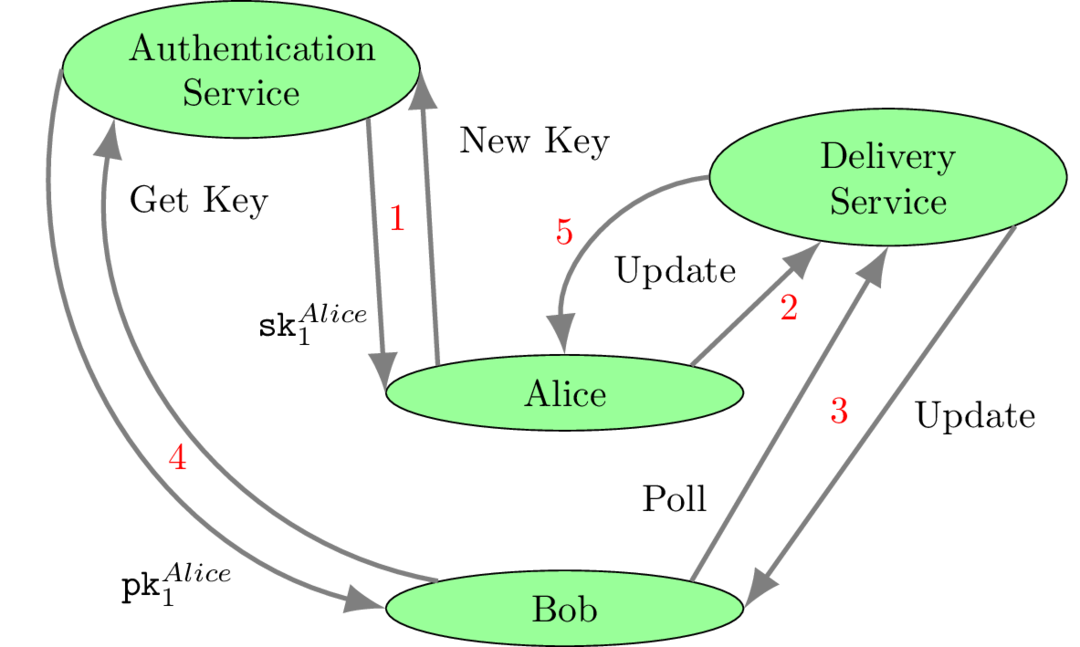
\includegraphics[width=0.8\textwidth]{./figures/Secure-Messaging-Update.png}
\end{figure}

The most scrutinized aspect of the \Abrev{MLS} specification involves the set of security guarantees that participants in a conforming a protocol can expect.
The security guarantees of \Abrev{MLS} includes many ``solved problems'' in the field of cryptography with respect to the \Abrev{ITM}; notably: end-to-end encryption \autocite{padlipsky1978limitations}, message confidentiality \autocite{17715}, message integrity \autocite{voydock1983security}, message authentication \autocite{jueneman1983message}, and membership authentication \autocite{chaum1985showing}.
However, \Abrev{MLS} also specifies interesting open problems related to \Abrev{FS} \autocite{gunther1989identity} and \Abrev{PCS} \autocite{cohn2016post} as security guarantees of the group key-agreement protocol.
Both \Abrev{FS} and \Abrev{PCS} have been researched with respect to \Abrev{SM}, producing provably secure as well as efficient constructions.
A popular example is the double-ratchet-based AXOLOTL algorithm \autocite{perrin2014axolotl} and its derivatives which are used by most \Abrev{SM} protocols.
The term ``ratchet,'' in a cryptographic context, refers to key derivation function which can be updated to derive the next key from the current key, but never derive the previous key from the current key.
Utilizing ratchets in the AXOLOTL and derivative protocols was essential for providing \Abrev{FS} and \Abrev{PCS}.
Interestingly, prior definitions of \Abrev{FS} introduced with the development of AXOLOTL were not defined generally enough to be directly used by \Abrev{MLS}.
\Abrev{MLS} defines a more general security guarantee for the multi-party notion of \Abrev{FS}, included in Section\ \ref{sec:forward-secrecy-with-updates}.
However, the requirement of \Abrev{FS} and \Abrev{PCS} laid out by the \Abrev{MLS} specification for a \Abrev{SGM} protocol has introduced a new area of research, as the double-ratchet-based algorithms do not directly map to multi-party communication.
Indeed, these \Abrev{MLS} security guarantees have been the chief focus of research related to \Abrev{MLS} and its iterative development.

Security guarantees are not the only concern of the \Abrev{MLS} specification.
For example, one can utilize a trivial protocol construction for \Abrev{SGM} by utilizing an existing \Abrev{SM} protocol, and forming a fully connected (finite) graph of bidirectional \Abrev{SM} communication channels between all \Abrev{SGM} participants.
Unsuprisingly, this trivial construction's control messages scale quadratically in the size of the communication group whenever the shared encryption key requires an update.
Maintaining key agreement with this trivial construction is not efficient.
Hence both security and efficiency are considerations in protocol construction.

The \Abrev{IETF} includes within \Abrev{MLS} efficiency goals \autocite{ietf-mls-architecture-07} for protocol constructions with respect to the size of the (finite) messaging group.
Three key efficiency distinctions which \Abrev{MLS} requires are that the number of control messages should be linear in group size, the size of control messages should be sub-linear in group size, and that group sizes up to 50,000 should be supported.
While efficient scaling up to a group comtaining 50,000 member is the target of all \Abrev{MLS} protocols, no guidance is given for larger groups.
One can assume that protocol efficiency may degrade above the target bound of 50,000 group members, but continued efficient scaling past this bound is preferable.
Taken in its entirely, the framework provided by \Abrev{MLS} is a foundational piece of achieving \Abrev{SGM} with well understood efficiency, security guarantees, and protocol design.


\hypertarget{sec:treekem-protocol}{%
\section{TreeKEM Protocol}\label{sec:treekem-protocol}}

The construction of scalable MSL protocols remains an area of open and active research, though the ``openness'' of this area closes each year.
There currently exist two proposed protocols which meet the definition of \Abrev{MLS} with various levels of security proofs as well as efficiency with respect to group size.
The first is Asynchronous Ratcheting Tree (ART) \autocite{cohn2018ends} described in 2018.
The second is TreeKEM \autocite{bhargavan:hal-02425247} similarly conceived in 2018, but thoroughly described in 2019.
The Internet Engineering Task Force has put its support behind the TreeKEM protocol along with many other corporate and government sponsors.
Consequently, research directed towards ART has stalled while developments for TreeKEM and its derivatives have progressed rapidly.
As the \Abrev{MLS} draft specification has gone through over a dozen revisions in the last half decade, the complimentary development and refinement of the TreeKEM protocol has significantly informed the direction and language of \Abrev{MLS}.
The verification work presented here will ignore ART and focus exclusively on the TreeKEM protocol.

TreeKEM provides functionality for achieving each of the six operations to be considered a \Abrev{SGM} protocol.
Additionally TreeKEM aims to satisfy both the efficiency goals and security guarantees of the \Abrev{MLS} specification.
Conformance with both of these definitions are a result of TreeKEM's construction.
The essence of TreeKEM is a protocol to generate continuous, fresh, shared, and secret random keys for use by group members.
The TreeKEM secret key material evolves over time in such a way that all group members maintain continuous agreement of the shared secret key.
A shared secret key is used to initiate a symmetric hash ratchet which defines a stream of nonce and key pairs for symmetric encryption using an \Abrev{AEAD} algorithm \autocite{bellare2003conventional, kohno2003cwc}.
Messages broadcast to the group are encrypted with an \Abrev{AEAD} algorithm using the the most recent nonce and key pair.
The stream is used until the shared secret key evolves, after which, a new stream is initiated using the evolved key.
Hash ratchet's produced by TreeKEM are analogous to double-ratchet based protocols in prior work, with the notable difference that, rather than using two ratchets for the two group members, TreeKEM uses a left balanced binary tree structure to define key agreement as a propagation from leaves of the tree to the root node, which supports an arbitrarily large number of group members instead of explicitly two members.
This generalization presented in TreeKEM is at the heart of constructing a protocol implementation satisfying the \Abrev{MLS} specification.
Unsurprisingly, this same generalization is appreciably linked to proving and verifying the \Abrev{FS} and \Abrev{PCS} security guarantees of TreeKEM.\@

\begin{figure}[ht!]
  \centering
  \caption[TreeKEM shared secret update.]{%
  \label{fig:CGKA-TreeKEM-Secrets}%
  An update operation initiated by the party at leaf \(v_0\): First, a random ``seed value'' \(s_0\) is chosen.
  Thereafter, a PRG is applied iteratively at every level \(i\) of \(v_0\)'s direct path in order to derive
  (i) a PKE secret key \(sk_i\) for that level (from which a public key can be computed using the key generation algorithm) and
  (ii) a seed \(s_{i+1}\) for the next level.
  Every seed \(s_i\) is encrypted using the public key of the corresponding co-path node \(v_{i-1}\).
  Sometimes, such a node can be blank, in which case \(s_i\) must be encrypted using the public keys of each node in the resolution, which is the smallest set of nodes covering all leaves in the subtree of \(v_{i-1}\).
  This ensures that all these nodes are able to compute the keys from \(v_i\) upward.
  The update secret \(I\) produced by such an update is the seed value \(s_d\) at the root.
  }%
  \copyrightbox[b]
  {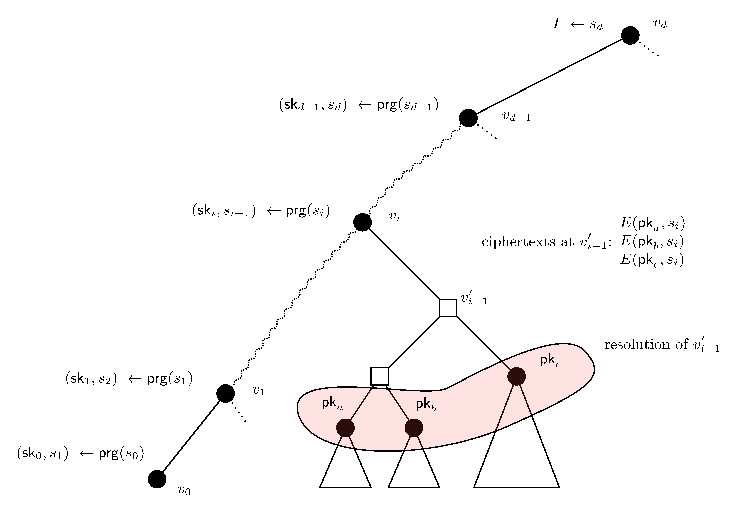
\includegraphics[width=\textwidth]{./figures/CGKA-TreeKEM-Secrets.eps}}
  {\CopyrightReuse{alwen2020security}}
\end{figure}

The TreeKEM protocol is based around a \Abrev{LBBT} \autocite{baerentzen2003left} shared by all participants.
Each leaf node in the tree contains the public key \autocite{rfc4949} of exactly one group member, with each group member being associated with a unique leaf in the tree.
Internal nodes of the tree contain a constructed public key, such that the private key is known to each group member in the associated sub-tree
The root of the tree contains a symmetric key \autocite{rfc4949} known to all group members.
Any member may force the evolution of the shared secret key if and only if they initiate adding a new group member, removing an existing group member, or the key update procedure.
In each case, the shared secret key at the root node is updated in the same manner.
The initiating member $v_{0}$ selects a random seed \autocite{rfc4949} value \(s_0\) and uses it to produce a public/secret key pair \((pk_0,sk_0)\) as well as a new seed value \(s_1\).
Member $v_{0}$ then encrypts the \(s_1\) with the public key of its sister leaf node.
Iteratively, member $v_{0}$ moves up the spine of the tree from their leaf node to the root node, using the seed value \(s_n\) to generate \((pk_n,sk_n,s_n)\) and encrypting \(s_n\) with the public key of the sister node on level \(n\) of the tree.
When member $v_{0}$ has propagated the changes to the root node, the final seed value \(s_r\) is determined to be the new shared secret key.
Note that each member of the group can derive the seed value required to update their copy of the shared key by decrypting the seed value \(s_n\) on the node prior to where the path from said member and the initiating member intersect.
Once each member has the requisite seed value, they each locally resume the iterative process of updating the tree and arrive at the same construction as that of the initiating member.
Note that each member updates their copy of the tree concurrently after receiving member $v_{0}$'s update instruction message from the \Abrev{DS}.
Concurrency issues and race conditions are obviated by the \Abrev{DS}'s guarantee of delivering messages to all group members in a consistent order.
For a visualization of this process, refer to Figure\ \ref{fig:CGKA-TreeKEM-Secrets}.


\hypertarget{sec:communication-epochs}{%
\section{Communication Epochs}\label{sec:communication-epochs}}

\begin{figure}[ht!]
  \centering
  \caption[Secure Messaging Epoch Timeline]{%
  \label{fig:Secure-Messaging-Timeline}%
  Secure Messaging Epoch Timeline
  }%
\resizebox{\textwidth}{!}{\subimport{../figures/}{Secure-Messaging-Timeline}}
\end{figure}

The temporality of \Abrev{SGM} protocols, as with the \Abrev{SM} protocols which proceeded them, is important to understanding how security of the protocol is defined.
Delineation of communication into discrete quanta referred to as ``epochs,'' is (generally) the way temporality is discussed when considering protocol security.
An illustration of epochs for a \Abrev{SM} protocol is included in Figure \ref{fig:Secure-Messaging-Timeline}, though the same deliniation applies to \Abrev{SGM} protocols as well.
Protocol epochs can be understood in terms of the \Abrev{SGM} usage.
A communication group is a set of two or more agents using multiple devices to engage in secure communication.
To initialize a group, members connect to the \Abrev{AS} and \Abrev{DS} providers which transmit the requisite credentials and values used for authentication of and encryption between the group members.
Using this initial information, the instigating group member begins the first encryption ``epoch'' by broadcasting control messages to all other group members.
The control message received by each group member provides instructions from which they can securely derive the initial shared symmetric key.
Subsequently, group members exchange messages with an enforced total ordering \autocite{halmos1960naive} mediated by the \Abrev{DS} and authenticated via the \Abrev{AS}, allowing for asynchronous communication with offline members while preventing the general sequencing issues and race conditions which arise from concurrency.
Additionally, any group member inititates a new encryption ``epoch'' by broadcasting a control message for one of the following operations:

\begin{itemize}
  \item add a member to the group
  \item remove a member from the group
  \item reset their continuously agreed upon symmetric encryption key
\end{itemize}

Advancing to a new epoch requires the creation of a new symmetric key known to all group members and secret to all other parties.
FSU (see Section \ref{sec:forward-secrecy-with-updates}) and \Abrev{PCS} for TreeKEM, as well as other \Abrev{SGM} protocols, are delineated in said epochs.
The inputs for a group member to generate the new symmetric key is referred to as an update secret.
An update secret is an intentionally abstract concept, defined as any cryptographic material stored by the group member required to process a control message which advanced the protocol from one epoch to the next, permitting the member to successfully generate the shared group key of the next epoch.
Each protocol may have a different specific form that update secret(s) take for a group member, but the interaction of group member update secrets with protocol control messages are the main focus of verifying security guarantees.


\hypertarget{sec:forward-secrecy-with-updates}{%
\section{Forward Secrecy with Updates}\label{sec:forward-secrecy-with-updates}}

\Abrev{FS} is a desirable security guarantee which offers protection in the case that a protocol's long-term secret key(s) are compromised.
The idea behind \Abrev{FS} is that even when all of a group member's current key material is compromised, messages delivered prior to the compromise are still secret.
\Abrev{FS} has been used in two-party key agreement communication protocols, including Transport Layer Security (TLS) \autocite{rfc2246, rfc4346, rfc5246, rfc8446} such as OpenSSL \autocite{openssl}, as well as \Abrev{SM} protocols such as the Signal Protocol \autocite{cohn2020formal}.
While the definition of \Abrev{FS} has been explored and made rigorously clear for two-party key agreement protocols, the notion of \Abrev{FS} requires extension in the multi-directional \Abrev{MLS} specification.
The following is the definition of \Abrev{FSU} in the multi-directional protocol context \autocite{alwen2020security} which has been adopted by \Abrev{MLS}.

\begin{definition}[Forward Secrecy with Updates]
If the state of any group member is leaked at some point, all previous shared keys remain hidden from the adversary.
\end{definition}


\hypertarget{sec:post-compromise-security}{%
\section{Post-compromise Security}\label{sec:post-compromise-security}}

Post-compromise Security (\Abrev{PCS}), within the context of bidirectional key agreement protocols, has been conflated with the definition of \Abrev{FS}.
However, within the multi-directional \Abrev{MLS} specification, the difference between \Abrev{FS} and \Abrev{PCS} has been separated to describe different security guarantee protocol when one or more of the protocol's long-term secret key(s) are compromised.
The idea behind \Abrev{PCS} is that no matter how many compromises of key material occur among the group members previously, once no new compromises occur, the group members will eventually reestablished secrecy through continued protocol usage.
The following definition of \Abrev{PCS} in the multi-directional protocol context \autocite{alwen2020security} which has been adopted by \Abrev{MLS}.

\begin{definition}[Post-compromise Security]
After every group member whose state was leaked inititates an epoch update, and that update instruction message is processed by all group members, the shared key becomes confidential again.
\end{definition}


\hypertarget{sec:CGKA}{%
\section{Continuous Group Key Agreement}\label{sec:CGKA}}

In the two-party case, a general notion of Continuous Key Agreement \autocite{alwen2019double} has been used to provide robust security guarantees such as forward secrecy and post-compromise security.
For \Abrev{SGM}, this same notion has been extended to \Abrev{CGKA} \autocite{alwen2020security} which is used as an abstraction reason about the \Abrev{MLS} security guarantees.
A continuous group key-agreement scheme is defined over a set of local member states $\gamma \in \Gamma$, a set welcome instruction messages for adding a member to a group $w \in W$, a set of update instruction messages $u \in U$, and a set of cryptographic secrets $i \in I$.
Additionally, a continuous group key-agreement scheme is require to define the following collection of algorithms:

\[ \CGKAdef = \left\{\,\Protocol{init},\, \Protocol{create},\, \Protocol{add},\, \Protocol{rem},\, \Protocol{upd},\, \Protocol{proc}\,\right\} \]

\begin{itemize}
\item \Protocol{init}   \(: ID \to \Gamma\)\\
  Given an \(ID\), output initial state \(\gamma\).
\item \Protocol{create} \(: \Gamma \times \overrightarrow{ID} \to (\Gamma, W)\)\\
  From state \(\gamma\) and list of \(ID\)s, output new state \(\gamma'\) and control message \(w\).
\item \Protocol{add}    \(: \Gamma \times ID \to (\Gamma, W, U)\)\\
  From state \(\gamma\) and \(ID\), output new state \(\gamma'\), control message \(w\) and control message \(u\).
\item \Protocol{rem}    \(: \Gamma \times ID \to (\Gamma, U)\)\\
  From state \(\Gamma\) and \(ID\), output new state \(\gamma'\) and a control message \(u\).
\item \Protocol{upd}    \(: \Gamma \to (\Gamma, U)\)\\
  From state \(\gamma\), output new state \(\gamma'\) and control message \(u\).
\item \Protocol{proc}   \(: \Gamma \times U \to (\Gamma, I)\)\\
  From state \(\gamma\) and control message \(u\), output new state \(\gamma'\) and update secret \(I\).
\end{itemize}

The abstract collection of algorithms \CGKAdef\ is used to maintain secure communications between a group of two or more participants.
In particular, any protocol which includes these algorithms can be used by a group to maintain continuous group key agreement of a shared secret key.
Each of the algorithms is performed atomically and locally by a group member.
The consistent ordering of messages supplied by the \Abrev{DS} ensures that each member will call algorithms in the same order.

Any group member can call any algorithm from \CGKAdef, producing new states \(\gamma \in \Gamma\) and either none, one, or both control messages \(w \in W,\; u \in U\).
These are ``welcome'' control messages \(w \in W\) for a new member entering the group and ``update'' control messages \(u \in U\) for existing members in the group instructing them how to update the shared symmetric key and advance to the next epoch.
The algorithm \(proc\) consumes control messages \(u \in U\) and produces a secret \(i \in I\).
Each call to \(proc\) by a group member facilitates \emph{processing} a control message.
Correspondingly, each call to \(proc\) by a group member ushers that user into a new epoch, where the secret \(i\) is the cryptographic secret required for the group member with \(ID\) to maintain \Abrev{CGKA} in the new epoch.
Group members who are offline, and unable to receive messages from the \Abrev{DS}, may fall an arbitrary number of epochs behind other members of the group.
However, when the lagging group member next polls the \Abrev{DS}, they will receive messages in a consistent order which instructs them how to incrementally advance to the current epoch while decrypting all broadcast messages which were transmitted during interstitial epochs.
In essence, the \Abrev{DS} mediates asynchornous epoch continuity among group members.

Because the communication is defined in terms of epochs, \Abrev{CGKA} should satisfy both Forward Secrecy and Post-compromise Security with respect to communication epochs.
The six requisite algorithms required for \CGKAdef\ can be produced by the functionality of the TreeKEM protocol.
For a visualization of each \CGKAdef\ algorithm defined using the functionality of TreeKEM, refer to Figure 4 of \autocite{alwen2020security}.
Using the six algorithms of \CGKAdef, the security guarantees in for TreeKEM are formulated in terms of a security game.


\hypertarget{sec:security-games}{%
\section{Security Games}\label{sec:security-games}}

A security game, in the context of cryptography and information security, involves an adversary \(\mathcal{A}\) which is permitted to perform some actions to observe or interact with a communication protocol.
The adversary \(\mathcal{A}\) ``wins'' the security game if they can acquire some information which is undesirable for the communicating parties.
Security games are designed with respect to a protocol, or class of protocols, and one or more security guarantees the protocol ought to preserve.
The winning condition(s) for \(\mathcal{A}\) within the security game are defined, by design, to occur if and only if \(\mathcal{A}\) can cause a violation of one or more security guarantees.
Often a security game includes one or more oracles.
An oracle is an agent in the game the adversary can query and to receive information or have an action performed on their behalf.
Oracles provide utility to an adversary, but importantly, the oracle does not explicitly inform the adversary how any queried information was produced nor how any queried action was performed.
The adversary must infer the effects of querying an oracle by observing messages broadcast to and from the \Abrev{DS}.

The same work which defines \Abrev{CGKA} also defines an oracle-based security game for \Abrev{CGKA}.
Each oracle is defined in terms of one or more of the algorithms from the \CGKAdef\ definition.
The adversary can query all of the game's oracles, and through the sequence of query's, the adversary uses the oracles to direct the execution of the \Abrev{CGKA} protocol.
In the game the adversary is given access to ten oracles to drive the execution of a \Abrev{CGKA} protocol.
The group members can only call the six \CGKAdef\ algorithms above, while the adversary can only query the ten oracles below.
However, there exists one oracle which corresponds to each of the six \CGKAdef\ algorithms, effectively giving the attacker comparable options to any group member in addition to the options provided by the remaining four oracles.
For a visualization of each oracles' semantics, refer to Figure\ \ref{fig:CGKA-Oracles}, reproduced from \autocite{alwen2020security}.
The \CGKAsec\ defines the following oracles:

\begin{itemize}

\item \Oracle{init}{}
Begins the \CGKAsec\ security game, initializing game and protocol state. Must be queried first.

\item \Oracle{create-group}{ID_0,\, ID_1,\, \dots,\, ID_n}
Creates an initial communication group to start the \CGKAsec\ game. Must be queried second.

\item \Oracle{add-user}{ID,\, ID^{'}}
\(mathcal{A}\) forces \(mathtt{ID}\) to initiate adding \(mathtt{ID}^{'}\) to the communication group.

\item \Oracle{remove-user}{ID,\, ID^{'}}
\(mathcal{A}\) forces \(mathtt{ID}\) to initiate removing \(mathtt{ID}^{'}\) from the communication group.

\item \Oracle{send-update}{ID}
\(mathcal{A}\) forces \(mathtt{ID}\) to initiate updating the shared key of the communication group.

\item \Oracle{deliver}{t,\, ID,\, ID^{'}}
\(mathcal{A}\) permits the \Abrev{DS} to deliver a message to \(mathtt{ID}^{'}\) which \(mathtt{ID}\) previously broadcast in epoch \(\mathtt{t}\).

\item \Oracle{no-del}{ID}
\(mathcal{A}\) forces \(mathtt{ID}\) to \emph{not} delete \(i \ in I\) values from this epoch and future epochs.

\item \Oracle{corr}{ID}
\(mathcal{A}\) learns the current state \(\gamma in \Gamma\) of \(mathtt{ID}\).

\item \Oracle{reveal}{t}
\(mathcal{A}\) learns the current shared key \(i in I\) of the communication group.

\item \Oracle{chall}{t}
\(mathcal{A}\) ends the \CGKAsec\ security game. Must be queried last.

\end{itemize}

\begin{figure}[ht!]
\centering
\caption[Oracles for the \CGKAsec]{%
\label{fig:CGKA-Oracles}%
Oracles for the \CGKAsec\ for a scheme \CGKAdef\ \(= \small\left(\,\Protocol{init},\, \Protocol{create},\, \Protocol{add},\, \Protocol{rem},\, \Protocol{upd},\, \Protocol{proc}\,\right)\).
}%
\copyrightbox[b]
{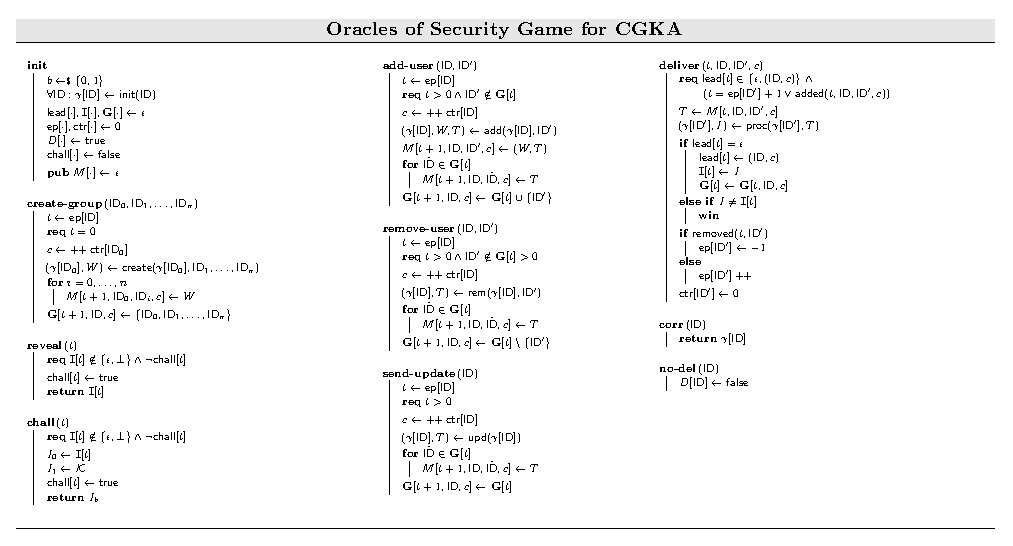
\includegraphics[width=\textwidth]{./figures/CGKA-Oracles.eps}}
{\CopyrightReuse{alwen2020security}}
\end{figure}

The first six oracles are call the \CGKAdef\ algorithms internally and can be intuitively thought of as thin wrappers exposed to \(\mathcal{A}\) for the corresponding algorithms from the \CGKAdef\ definition.
Importantly, these oracles encapsulate from the adversary the stateful production and consumption of group member state values \(\gamma \in \Gamma\) as well as the emission of secret key material values \(i \in I\).
Control messages \(w \in W\) and \(u \in U\) are still broadcast across the network and assumed to be intercepted by the adversary.
The definition of control messages within the TreeKEM protocol dictates that messages are are authenticated by the group members, which justifies the absence of an oracle permitting the adversary to change or replay intercepted control messages in the \Abrev{CGKA} game.

Despite the encapsulation, querying these oracles permits the adversary to both perform and observe ``side effects'' related to the protocol's execution.
Side channel information gained in querying oracles is dependent on the protocol with which the \CGKAsec\ is being played.
Hence, many propositions regarding the \CGKAsec\ semantics can only be correctly reasoned about when the protocol under consideration is also specified.
One semantic which is invariant of a specific protocol, emerges from querying the \Oracle{add-user}{}, \Oracle{remove-user}{}, and \Oracle{send-update}{} oracles, conferring onto the adversary the ability to guide the protocol execution by instructing group members to begin new epochs on whichever terms the adversary considers favorable.
Likewise the \Oracle{deliver}{} oracle permits the adversary to control when each user receives control messages and subsequently advances to the next epoch.
Because the adversary has access to the \Oracle{deliver}{} oracle, it does not matter who, adversary or group member, attempts to initiate a new epoch, ultimately the adversary decides via querying the \Oracle{deliver}{} oracle which epoch-initiating control messages are processed by the group.
Phrased differently, multiple new epochs can be concurrently initiated either from a group member calling the \textbf{add}, \textbf{rmv}, or \textbf{upd} algorithm from \CGKAdef, or from the adversary querying the \Oracle{add-user}{}, \Oracle{remove-user}{}, or \Oracle{send-update}{} oracles, but regardless of the epoch initiation attempt's origin, the adversary chooses via querying the \Oracle{deliver}{} oracle which of the possible initiation attempts is definitively processed by the group as the next epoch.

The \Abrev{DS} is guaranteed by the \Abrev{MLS} specification to provide all parties with a consistent presentation of messaging in and between epochs.
Note that when the adversary selects the terms under which the epoch transitions from \(t\) to \(t+1\), the \Abrev{DS} is compelled to \emph{not} deliver any other control messages attempting to transition from \(t\) to \(t+1\), as doing so would provide an inconsistent view of the protocol evolution.
Hence, any messages received by the \Abrev{DS} but have not yet been delivered to the recipient must be continuously checked and potentially discarded if they would present an inconsistent message ordering within an epoch or present an interleaving of epoch transitions.
An important consequence of maintaining this consistent view within the context of the adversarial \Abrev{CGKA} game is that, when the adversary queries the \Oracle{deliver}{} oracle enabling a chosen epoch transition from \(t\) to \(t+1\), the \Abrev{DS} must discard all other epoch transition messages with originated in a previous epoch.
By judiciously querying the \Oracle{add-user}{}, \Oracle{remove-user}{}, \Oracle{send-update}{}, and \Oracle{deliver}{} oracles, the adversary can effectively decide the protocol evolution, choosing which epoch transition they find desirable to be processed by the group members, and compelling the \Abrev{DS} to discard all other potential epoch transitions within the deliver queue.

The final four oracles exist to provide the adversary with means to gain undue knowledge of secret aspects of the \Abrev{CGKA} protocol.
The \Oracle{no-del}{} oracle forces the specified user to \emph{not} delete old key material when advancing to a new epoch.
The \Oracle{corr}{} oracle ``corrupts'' the specified user, revealing the user's key material to the adversary. Note that if \Oracle{no-del}{} is called before \Oracle{corr}{} on the same user, the adversary can learn the key material from multiple epochs!
The \Oracle{reveal}{} oracle produces the group's shared symmetric key of the specified epoch for the adversary.
The \Oracle{chall}{} oracle allows the adversary to signal that they believe that they have succeeded in violating the \Abrev{CGKA} protocol's security and the game should immediately cease so the adversary can provide proof of their successful attack by demonstrating \emph{advantage}.

Note that the requisite query to the \Oracle{init}{} oracle flips a random bit \(b\) uniformly at random and this result remains constant for the entirety of the game.
The random result assigned to \(b\) bit is used for the traditional ``real-or-random'' challenges in security games, in which the adversary must distinguish whether they are observing the actual cryptographic protocol or random information being transmitted.
If and only if \(b=1\) will the real control messages be broadcast across the network for the adversary to intercept when querying \Oracle{create-group}{}, \Oracle{add-user}{}, \Oracle{remove-user}{}, and \Oracle{send-update}{} oracles.
Similarly if and only if \(b=1\) will the real member states and update secrets be revealed to the adversary when querying the \Oracle{corr}{} and \Oracle{reveal}{} oracles.
When \(b=0\), random values are instead broadcast and revealed to the adversary when querying the oracles.
The goal of the adversary is to demonstrate advantage by discriminating the value of \(b\) with probability greater than \(\frac{1}{2}\).

An adversary demonstrating \emph{advantage} is defined by the \CGKAsec\ as a parameterized expression involving oracles of the game.
A tuple \((T, C, N)\) parameterizes the adversary \(\mathcal{A}\), with \(T \in \left[1, \infty \right]\), \(C \in \left[0, T \right]\), and \(N \in \left[2, \infty \right]\).
The \(T\) value indicates that the protocol runs in at most \(T\) epochs, during which time the \(\mathcal{A}\) can make at most \(C\) challenge queries, and the total unique group members of the protocol can never exceed \(N\).
Some security games, \CGKAsec\ included, provide oracles which permit a sequence of queries that can quite obviously and trivially allow an adversary to deduce the value of \(b\).
To correct for these sequences of queries, there exists a predicate \textbf{\texttt{P}}, which indicates that a trivial ``attack'' did not occur via oracle queries.
For security games with no such sequence of queries, the predicate \textbf{\texttt{P}} is always \(\top\).
More nuanced security games utilize predicate \textbf{\texttt{P}} to guard against a trivial sequence of queries from the adversary.
The \((T, C, N)\)-adversary \(\mathcal{A}\) demonstrates \emph{advantage} by ending the game via a query to the \Oracle{chall}{} oracle, winning the \CGKAsec, if and only if:

\begin{enumerate}
\item \(\mathcal{A}\) correctly determines the value random bit \(b\).
\item The predicate \textbf{\texttt{P}} evaluates to \(\top\).
\end{enumerate}
\vspace{\parsep}

\begin{definition}[\Abrev{CGKA} advantage]\label{def:CGKA-Advantage}
The advantage demonstrated by $\mathcal{A}$ is defined as,
\[ \normalfont{\textbf{Adv}}\left\{\CGKAdef,\textbf{\texttt{P}}\right\}(\mathcal{A})  = \left|\; \Pr\left[ \,\mathcal{A}\text{ wins}\, \right] - \frac{1}{2} \;\right| \]
\end{definition}

\begin{definition}[Non-adaptive $(T, C, N, \textbf{\texttt{P}}, \epsilon)$ \Abrev{CGKA} Security]\label{def:CGKA-Security}
A \Abrev{CGKA} protocol is said to be secure if and only if for all $(T, C, N)$-adversaries $\mathcal{A}$,
\[ \normalfont\textbf{Adv}\left\{\CGKAdef,\textbf{\texttt{P}}\right\}(\mathcal{A}) \leq \epsilon \]
\end{definition}

The \Abrev{CGKA} algorithms, security game, and \emph{Non-adaptive} \((T, C, N, \textbf{\texttt{P}}, \epsilon)\) \emph{\Abrev{CGKA} Security} definition are integral to the verification work presented in the subsequent chapters.
Chapter\ \ref{sec:methodology} will use the security definition to parameterize and constrain the verification methodology presented.
In a similar manner, the definition and understanding of \emph{Non-adaptive} \((T, C, N, \textbf{\texttt{P}}, \epsilon)\) \emph{\Abrev{CGKA} Security} will be extensively relied upon in Chapter\ \ref{sec:model-formalization} when constructing the model encoding of TreeKEM.\@
This reliance extends to the discussions in Section\ \ref{sec:game-adaptations} related to utilizing explicit state model checking when modeling and verifying TreeKEM
as well as in Section\ \ref{sec:game-oracles} modeling the translations of the \CGKAsec\ oracles explicitly for TreeKEM.\@
Additionally, the modeling of random \(b\) and adversary advantage will be elaborated on in Section\ \ref{sec:game-adaptations}.
Subsequently Section\ \ref{sec:LTL-security} presents definitions of the predicate \textbf{\texttt{P}} for prohibiting ``trivial attacks'' explicitly related to TreeKEM and the \Abrev{CGKA} game as described by \autocite{alwen2020security}.


\hypertarget{sec:concluding-abstraction}{%
\section{Concluding Abstraction}\label{sec:concluding-abstraction}}

It is worth noting the relationship between the preliminary definitions explored thus-far.
\Abrev{SGM} is a description of the high-level use case.
\Abrev{CGKA} is a class of protocols supporting the requisite algorithms, which by definition must facilitate \Abrev{SGM}.
The \Abrev{MLS} specification is a standardization of which protocols may conform to and satisfy the \Abrev{SGM} use case, necessarily maintains continuous group key agreement as defined by \Abrev{CGKA}, as well as provides efficiency and scalability guarantees.
TreeKEM is a specific cryptographic protocol which conforms to the \Abrev{MLS} specification.
There is a clear sub-setting relationship between these abstract concepts illustrated in Figure\ \ref{fig:venn-protocols}, and in future descriptions the layer of abstraction from which a definition was defined may be elided.

\begin{figure}
\centering
\caption{\label{fig:venn-protocols}Specificity relationship between preliminary definitions}
\resizebox{0.5\textwidth}{!}{\subimport{../figures/}{venn-protocols}}
\end{figure}

The definition of \Abrev{CGKA} and the construction of the \CGKAsec\ offers an abstraction between the protocol specific implementation and the desired security guarantees of \Abrev{FSU} and \Abrev{PCS} specified by \Abrev{MLS}.
An equivalence proof of non-adaptive \Abrev{CGKA} security definition\ \ref{def:CGKA-Security} with \Abrev{FSU} and also with \Abrev{PCS} accompanies its original description \autocite{alwen2020security}.
The verification work with follows relies on the equivalence proof in order to soundly use \Abrev{CGKA} as a verifiable abstraction.
The equivalence proof results in the corollary that an adversary playing the \CGKAsec\ can only gain advantage by exploiting side-channel attack on the given \Abrev{CGKA}-conforming protocol.

Consider a model \CGKAmod{}{}{} of the \CGKAsec.
To formulate arbitrary propositions regarding the model, \CGKAmod{}{}{} must be parameterized by a given \Abrev{CGKA}-conforming protocol \(\mathtt{P}\), denoted by \CGKAmod{P}{}{}.
utilizing the equivalence proof, a verification result of \CGKAmod{P}{}{} which verifies \Abrev{FSU} and \Abrev{PCS} at the abstraction level, will consequently verify the \Abrev{FSU} and \Abrev{PCS} security guarantees for the defined protocol \(\mathtt{P}\).
Operating at this selected level of abstraction is powerful, providing \(\mathcal{M}_{\texttt{CGKA}}\) as verification framework for a whole class of current and future protocols.
However, the \Abrev{CGKA} abstraction and model \CGKAmod{P}{}{} cannot verify that a given implementation of a protocol \(\mathtt{P}\) is defect-free implementation.
Additionally, the \Abrev{CGKA} abstraction and model \CGKAmod{P}{}{} are dependent on the protocol parameter \(P\).

This work reduces future verification burdens for all \Abrev{CGKA}-conforming protocol implementations \(P\) in the following ways.
First, a separate and specific verification effort is required to prove that the implementation of \(\mathtt{P}\) provides a correct version of the \Abrev{CGKA} algorithms.
Second, the model \CGKAmod{}{}{} must be parameterized by \(P\) and then verified.
The parameterizable model \CGKAmod{}{}{} produced during and described within this work exposes a polymorphic interface for a protocol to express side channel information the adversary learns from querying oracles.
To produce \CGKAmod{P}{}{}, the interface methods must be instantiated for \(P\) as well an encapsulated representation of the adversary knowledge which is maintained via the interface.
After performing these two verification efforts, if a predicate \(\varphi\) is verified for \CGKAmod{P}{}{}, then the predicate \(\varphi\) holds for \(P\).

Even operating without a formal model, the \Abrev{CGKA} abstraction is a powerful tool.
Accompanying the description of \Abrev{CGKA}, \CGKAdef, and the \CGKAsec\ the authors also include an application of mathematically analyzing TreeKEM with the \CGKAsec.
The result of the analysis was a constructive counter-example demonstrating that TreeKEM, as originally defined, is \emph{not} \Abrev{FS}.
Following the revelation of TreeKEM's deficiency the same authors present a new definition of TreeKEM, substituting the use of a standard PKE cryptographic primitive with UPKE, which remedies the defect and regains the \Abrev{FSU} security guarantee for TreeKEM.\@

The proceeding work will perform verification of the two versions of TreeKEM.\@
All results presented by this work assume that the TreeKEM algorithms' implementations are correct.
Verification of TreeKEM will consider both the original definition of TreeKEM as well as the remedied version of TreeKEM, denoted by \VersionOne\ and \VersionTwo; respectively.
Using the notation introduced above, the \Abrev{CGKA} abstraction for TreeKEM produces the \CGKAmod{\VersionOne}{}{} and \CGKAmod{\VersionTwo}{}{} models, which will both be verified.
Verifying the correctness of the \Abrev{CGKA} algorithm implementations for each TreeKEM version is beyond the scope of this work.
Rather, it is assumed that a given an implementation of the specified TreeKEM version \(\mathtt{P}\) provides defect-free algorithms.
If the defect-free algorithm assumption holds, then a verification of the \Abrev{FSU} or \Abrev{PCS} security guarantee for \CGKAmod{P}{}{} also verifies the security guarantee for corresponding TreeKEM version implementation.
The verification hypotheses are depicted in Table\ \ref{tab:verification-hypotheses}.

\begin{table}[ht!]                                                                                                                      
\caption{%
\label{tab:verification-hypotheses}%
Verification Hypotheses of \CGKAmod{P}{}{}.
}%
\subimport{../tables/}{verification-hypotheses}
\end{table}
